\chapter{Resultados e Discussão}
\label{chp:resultados}

Este capítulo apresenta os resultados experimentais da tarefa de regressão supervisionada nas três configurações do pipeline, todas integralmente concluídas, e a análise de interpretabilidade via SHAP sobre os melhores modelos da Config~C. Os resultados de Config~A (linha de base, atributos brutos, 11 modelos), Config~B (MLP profundo com busca de arquitetura via Optuna, atributos brutos) e Config~C (física informada, atributos brutos mais os oito físico-derivados, 12 modelos) são reportados com MAE, RMSE, $R^2$ e fração de predições dentro da tolerância industrial ($w_\text{tol}$). A comparação A~vs.~C é testada com o teste de Wilcoxon com postos assinados sobre os 1.500 erros absolutos pareados do conjunto de teste\,\cite{demsar2006statistical}. Ao total foram treinados e avaliados 33 combinações (modelo $\times$ alvo) para a Config~A, 3 para a Config~B e 36 para a Config~C, perfazendo 72 modelos otimizados via Optuna com 20 \textit{trials} cada. O tempo total, da geração de dados aos resultados de SHAP e circularidade aqui reportados, foi de aproximadamente 10\,h\,29\,min no ambiente computacional descrito no Capítulo~\ref{chp:capitulo4}, com o treinamento dos modelos (etapa 3) dominando o tempo total e a busca de arquitetura profunda do MLP (Configs~B e~C) sendo a mais custosa por modelo individual.

\section{Config~A: Linha de Base com Atributos Brutos}
\label{sec:resultados-A}

Os resultados completos de Config~A são exibidos na Tabela~\ref{tbl:resultados_configA}. MAE em negrito indica cumprimento do limiar industrial.

\begin{table}[H]
\caption{Config~A --- atributos brutos, 11 modelos. MAE em negrito: cumpre limiar industrial ($T_\text{final} \leq 10\,^\circ\text{C}$; $[\text{C}]_\text{final} \leq 0{,}020\,\%$; $[\text{P}]_\text{final} \leq 0{,}003\,\%$)~\cite{zhou2024bof,bae2020bof}. $w_\text{tol}$: fração de predições dentro da tolerância. Dataset $N=10{.}000$; partição 70/15/15\,\%; Optuna 20 \textit{trials}/modelo/alvo.}
\label{tbl:resultados_configA}
\centering
\footnotesize
\setlength{\tabcolsep}{4pt}
\begin{tabular}{lrrrrrrrrrr}
\hline
\textbf{Modelo} &
  \multicolumn{3}{c}{$T_\text{final}$ (°C)} &
  \multicolumn{3}{c}{$[\text{C}]_\text{final}$ (\%)} &
  \multicolumn{3}{c}{$[\text{P}]_\text{final}$ (\%)} \\
\cline{2-4}\cline{5-7}\cline{8-10}
 & MAE & $R^2$ & $w_\text{tol}$ & MAE & $R^2$ & $w_\text{tol}$ & MAE & $R^2$ & $w_\text{tol}$ \\
\hline
Ridge      & 23,91 & 0,367 & 22,2\,\% & \textbf{0,0156} & 0,711 & 66,3\,\% & 0,00326 & 0,601 & 53,9\,\% \\
Lasso      & 23,91 & 0,367 & 22,2\,\% & \textbf{0,0156} & 0,711 & 66,5\,\% & 0,00327 & 0,600 & 53,3\,\% \\
ElasticNet & 23,91 & 0,367 & 22,2\,\% & \textbf{0,0156} & 0,711 & 66,5\,\% & 0,00326 & 0,601 & 54,1\,\% \\
RF         & 23,45 & 0,351 & 25,0\,\% & \textbf{0,0093} & 0,823 & 85,1\,\% & 0,00304 & 0,641 & 58,6\,\% \\
GBM        & 23,43 & 0,342 & 26,4\,\% & \textbf{0,0093} & 0,816 & 84,7\,\% & 0,00301 & 0,641 & 59,1\,\% \\
XGBoost    & 23,24 & 0,356 & 25,5\,\% & \textbf{0,0096} & 0,825 & 84,9\,\% & 0,00302 & 0,641 & 59,1\,\% \\
LightGBM   & 23,08 & 0,338 & 29,7\,\% & \textbf{0,0088} & 0,831 & 85,7\,\% & 0,00300 & 0,646 & 59,4\,\% \\
CatBoost   & 23,25 & 0,365 & 26,5\,\% & \textbf{0,0094} & 0,832 & 83,7\,\% & \textbf{0,00299} & 0,648 & 58,9\,\% \\
SVR        & 21,86 & 0,347 & 35,9\,\% & \textbf{0,0129} & 0,771 & 78,1\,\% & 0,00348 & 0,546 & 49,3\,\% \\
KNN        & 26,00 & 0,254 & 18,8\,\% & \textbf{0,0157} & 0,635 & 67,9\,\% & 0,00355 & 0,546 & 46,9\,\% \\
MLP        & 24,88 & 0,309 & 22,1\,\% & \textbf{0,0091} & 0,840 & 84,5\,\% & 0,00314 & 0,626 & 55,3\,\% \\
\hline
\end{tabular}
\end{table}

Os resultados da Config~A revelam uma hierarquia de dificuldade marcada entre os três alvos. $[\text{C}]_\text{final}$ é o alvo mais bem capturado pelos atributos brutos: todos os onze modelos atendem ao limiar de 0{,}020\,\%, com os ensembles de árvore e o MLP (RF, GBM, XGBoost, LightGBM, CatBoost, MLP) alcançando MAE entre 0{,}0088\,\% e 0{,}0096\,\% e $R^2$ até 0{,}840. Isso indica que as variáveis brutas --- especialmente $[\text{C}]_\text{hm}$ e $\dot{V}_{\text{O}_2}$ --- já codificam suficientemente a relação exponencial de descarburação.

$T_\text{final}$ é o alvo discriminante: nenhum dos onze modelos atinge o limiar de $10\,^\circ\text{C}$, com MAE variando entre $21{,}86\,^\circ\text{C}$ (SVR) e $26{,}00\,^\circ\text{C}$ (KNN) e $R^2$ entre 0{,}254 e 0{,}367. Este resultado merece interpretação cuidadosa: o limiar de $10\,^\circ\text{C}$ adotado na literatura~\cite{xia2024dmpinn,bae2020bof} pressupõe a disponibilidade de informação temporal durante o sopro (perfis de off-gas, medições de sublança intermediárias), que são inacessíveis a um modelo estático pré-sopro como o desta dissertação. A questão não é se os modelos falharam, mas sim qual é o limite informacional-teórico da predição com variáveis exclusivamente pré-sopro. O $R^2$ entre 0{,}25 e 0{,}37 reflete, em parte, a variância irredutível imposta por $\eta_\text{eff} \sim \mathcal{N}(0{,}64;\,6\%)$, uma grandeza estocástica por corrida não observável nas features de entrada --- análogo ao ruído de Bayes em classificação\,\cite{bishop2006prml,goodfellow2016deep}; essa variância estabelece um teto teórico que nenhum modelo supervisionado pode ultrapassar com os atributos disponíveis. Mas parte do $R^2$ reportado também é inflada pela censura de $T_\text{final}$ nos limites da faixa-alvo (Capítulo~\ref{chp:capitulo4}, $40{,}5\,\%$ das amostras): recalculando sobre o subconjunto de teste não saturado, o $R^2$ do SVR (Config~A) cai de $0{,}347$ para $0{,}240$, enquanto o MAE se mantém praticamente inalterado ($21{,}86\,^\circ\text{C}$ vs.\ $22{,}00\,^\circ\text{C}$) --- ou seja, a censura reduz artificialmente a variância total a explicar sem tornar a predição pontual mais fácil.

$[\text{P}]_\text{final}$ constitui o segundo alvo crítico: apenas o CatBoost atinge o limiar de 0{,}003\,\% (MAE~$=0{,}002993\,\%$, margem mínima), com os demais ensembles em MAE~$\approx 0{,}0030\,\%$ --- fração de um por cento acima --- e $w_\text{tol}$ entre 58{,}6\,\% e 59{,}4\,\%. O $R^2$ (0{,}55--0{,}65) reflete a dificuldade de inferir a basicidade efetiva da escória sem o atributo combinado \texttt{slag\_basicity}: a remoção de fósforo é função fortemente não-linear desta variável~\cite{bae2020bof,chattopadhyay2022hybrid}.

A convergência dos três modelos lineares (Ridge, Lasso, ElasticNet) em desempenho quase idêntico confirma que o gargalo nessa família é estrutural --- incapacidade de capturar interações de segunda ordem --- e não hiperparamétrico. Esse é precisamente o cenário onde atributos físico-derivados pré-computados têm maior impacto esperado~\cite{willard2020integrating,chattopadhyay2022hybrid}.


\section{Config~B: MLP Profundo com Atributos Brutos}
\label{sec:resultados-B}

A Config~B avalia se a profundidade arquitetural do MLP, com busca automática de número de camadas e neurônios via Optuna, é suficiente para superar os ensembles da linha de base sem atributos físico-derivados. Os resultados são exibidos na Tabela~\ref{tbl:resultados_configB}.

\begin{table}[H]
\caption{Config~B --- MLP profundo (\texttt{mlp\_deep}) com atributos brutos. Busca de arquitetura via Optuna (20 \textit{trials}); os demais protocolos são idênticos à Config~A.}
\label{tbl:resultados_configB}
\centering
\footnotesize
\setlength{\tabcolsep}{5pt}
\begin{tabular}{lrrrrrrrrrr}
\hline
\textbf{Modelo} &
  \multicolumn{3}{c}{$T_\text{final}$ (°C)} &
  \multicolumn{3}{c}{$[\text{C}]_\text{final}$ (\%)} &
  \multicolumn{3}{c}{$[\text{P}]_\text{final}$ (\%)} \\
\cline{2-4}\cline{5-7}\cline{8-10}
 & MAE & $R^2$ & $w_\text{tol}$ & MAE & $R^2$ & $w_\text{tol}$ & MAE & $R^2$ & $w_\text{tol}$ \\
\hline
MLP$_\text{deep}$ & 24,03 & 0,342 & 23,5\,\% & \textbf{0,0090} & 0,839 & 84,5\,\% & 0,0032 & 0,608 & 55,3\,\% \\
\hline
\end{tabular}
\end{table}

A Config~B não supera os melhores modelos da Config~A em nenhum dos três alvos: o MLP profundo obtém MAE$_{T} = 24{,}03\,^\circ\text{C}$ contra $21{,}86\,^\circ\text{C}$ do SVR --- o melhor modelo da Config~A para este alvo --- e frente aos ensembles de árvore (23{,}08--23{,}45\,\textdegree C) também não há ganho. Para $[\text{C}]_\text{final}$ e $[\text{P}]_\text{final}$ o MLP profundo é comparável, mas não superior, aos modelos de boosting. Esse resultado é consistente com a literatura sobre dados tabulares de domínio industrial, onde gradiente-boosting tende a superar redes neurais rasas e profundas quando o número de amostras é da ordem de $10^4$ e as relações entre variáveis não têm estrutura espacial ou temporal explorada por convoluções ou recorrências~\cite{grinsztajn2022tree,shwartz2022tabular}. A implicação prática é que, no domínio BOF com dados tabulares estáticos, investir em profundidade arquitetural sem incorporar conhecimento físico não produz ganho preditivo.


\section{Config~C: Física Informada com Oito Atributos Físico-Derivados}
\label{sec:resultados-C}

A Config~C expande o espaço de atributos com os oito físico-derivados descritos no Capítulo~\ref{chp:capitulo4}. Os resultados completos são exibidos na Tabela~\ref{tbl:resultados_configC}.

\begin{table}[H]
\caption{Config~C --- atributos brutos + 8 físico-derivados, 12 modelos. Mesmas convenções da Tabela~\ref{tbl:resultados_configA}.}
\label{tbl:resultados_configC}
\centering
\footnotesize
\setlength{\tabcolsep}{4pt}
\begin{tabular}{lrrrrrrrrrr}
\hline
\textbf{Modelo} &
  \multicolumn{3}{c}{$T_\text{final}$ (°C)} &
  \multicolumn{3}{c}{$[\text{C}]_\text{final}$ (\%)} &
  \multicolumn{3}{c}{$[\text{P}]_\text{final}$ (\%)} \\
\cline{2-4}\cline{5-7}\cline{8-10}
 & MAE & $R^2$ & $w_\text{tol}$ & MAE & $R^2$ & $w_\text{tol}$ & MAE & $R^2$ & $w_\text{tol}$ \\
\hline
Ridge          & 23,90 & 0,368 & 21,7\,\% & \textbf{0,0131} & 0,766 & 77,2\,\% & 0,00324 & 0,602 & 53,9\,\% \\
Lasso          & 23,90 & 0,367 & 22,1\,\% & \textbf{0,0134} & 0,763 & 76,0\,\% & 0,00327 & 0,600 & 53,3\,\% \\
ElasticNet     & 23,90 & 0,367 & 22,1\,\% & \textbf{0,0131} & 0,766 & 76,9\,\% & 0,00325 & 0,602 & 53,9\,\% \\
RF             & 23,51 & 0,348 & 24,7\,\% & \textbf{0,0087} & 0,838 & 85,1\,\% & \textbf{0,00293} & 0,662 & 61,1\,\% \\
GBM            & 23,33 & 0,344 & 26,9\,\% & \textbf{0,0087} & 0,840 & 85,8\,\% & \textbf{0,00294} & 0,663 & 60,1\,\% \\
XGBoost        & 23,20 & 0,359 & 26,5\,\% & \textbf{0,0090} & 0,838 & 86,3\,\% & \textbf{0,00294} & 0,661 & 59,8\,\% \\
LightGBM       & 23,31 & 0,339 & 26,5\,\% & \textbf{0,0088} & 0,840 & 86,1\,\% & \textbf{0,00294} & 0,662 & 59,4\,\% \\
CatBoost       & 23,16 & 0,365 & 26,7\,\% & \textbf{0,0086} & 0,843 & 85,9\,\% & \textbf{0,00293} & 0,664 & 60,2\,\% \\
SVR            & 22,15 & 0,348 & 34,5\,\% & \textbf{0,0099} & 0,820 & 82,7\,\% & 0,00348 & 0,538 & 49,2\,\% \\
KNN            & 25,84 & 0,265 & 17,3\,\% & \textbf{0,0131} & 0,713 & 73,8\,\% & 0,00356 & 0,547 & 47,1\,\% \\
MLP            & 27,37 & 0,120 & 21,1\,\% & \textbf{0,0090} & 0,842 & 85,7\,\% & \textbf{0,00297} & 0,645 & 58,9\,\% \\
MLP$_\text{deep}$ & 25,06 & 0,269 & 22,9\,\% & \textbf{0,0088} & 0,844 & 85,5\,\% & 0,0030 & 0,646 & 58,9\,\% \\
\hline
\end{tabular}
\end{table}

Os resultados da Config~C evidenciam um padrão assimétrico entre os três alvos, que constitui a principal descoberta experimental desta dissertação.

Para $[\text{C}]_\text{final}$, os oito atributos físico-derivados produzem melhoria estatisticamente significativa pelo teste de Wilcoxon em 10 dos 11 pares A~vs.~C ($p < 0{,}05$; Tabela~\ref{tbl:wilcoxon_detail}) --- a exceção é o LightGBM ($p = 0{,}441$), cujo desempenho já era o melhor da Config~A e deixa pouca margem de ganho. Os modelos de gradiente-boosting atingem MAE entre 0{,}0086\,\% (CatBoost) e 0{,}0090\,\% (XGBoost) --- redução de até 8{,}7\,\% em relação à Config~A no CatBoost, mas de apenas 0{,}8\,\% no LightGBM (o único par não significativo desta lista) --- com $R^2$ até 0{,}843. Atributos como \texttt{o2\_efficiency} e \texttt{decarb\_rate} codificam relações termodinâmicas que os ensembles de árvore passam a acessar diretamente como divisões de nó, em vez de precisar reaprendê-las a partir de interações entre variáveis brutas~\cite{willard2020integrating,shao2024hybrid}.

Para $[\text{P}]_\text{final}$, oito dos 11 pares mostram melhoria significativa ($p \leq 0{,}028$; Tabela~\ref{tbl:wilcoxon_detail}) --- Lasso, SVR e KNN são as exceções não-significativas. O ganho mais notável é prático, não apenas estatístico: seis modelos (RF, GBM, XGBoost, LightGBM, CatBoost, MLP) passam a atender ao limiar industrial de 0{,}003\,\%, contra apenas um (CatBoost, por margem mínima) na Config~A. O melhor resultado é o CatBoost, com MAE~$= 0{,}002926\,\%$ --- $2{,}5\,\%$ abaixo do limiar. A incorporação de \texttt{slag\_basicity}, que condensa (CaO + MgO)/$\text{SiO}_2$ em um único atributo, desloca uma fração substancial dos modelos de fósforo para dentro da faixa de aceitação industrial~\cite{bae2020bof,chattopadhyay2022hybrid}.

O caso mais chamativo da Config~C é o MLP em $T_\text{final}$: seu MAE sobe de $24{,}88\,^\circ\text{C}$ (Config~A) para $27{,}37\,^\circ\text{C}$ (Config~C), com $R^2$ caindo de $0{,}309$ para $0{,}120$ --- a maior degradação observada em toda a comparação. De forma mais geral, nenhum modelo da Config~C apresenta melhoria estatisticamente significativa para $T_\text{final}$ (Tabela~\ref{tbl:wilcoxon_detail}): os atributos físico-derivados não resolvem o gargalo deste alvo. Como o teste de Wilcoxon aqui aplicado é unilateral (testa apenas se C é melhor que A), ele não pode, por construção, atestar significância estatística para uma piora; a degradação do MLP é, portanto, relatada como observação descritiva direta das métricas (não como resultado de teste de hipótese) e é consistente com dificuldades conhecidas de convergência de redes neurais quando a dimensionalidade de entrada aumenta sem crescimento proporcional do conjunto de treino~\cite{goodfellow2016deep,grinsztajn2022tree}. Esses resultados confirmam o teto informacional discutido na Seção~\ref{sec:resultados-A}: a variância irredutível de $\eta_\text{eff}$ limita o ganho possível para $T_\text{final}$ independentemente da estratégia de atributos.

Os modelos lineares apresentam ganho relevante em $[\text{C}]_\text{final}$ na Config~C ($\Delta$MAE entre $-0{,}0022$ e $-0{,}0025\,\%$, todos significativos), confirmando que os atributos físico-derivados linearizam interações antes inacessíveis a regressores sem termos de interação explícitos. Para $T_\text{final}$, o ganho linear é nulo; para $[\text{P}]_\text{final}$, Ridge e ElasticNet melhoram significativamente, mas Lasso não --- provavelmente por zerar o coeficiente de algum atributo físico-derivado durante a regularização $L_1$.


\section{Comparação Estatística A~vs.~C}
\label{sec:comparacao-ac}

A Tabela~\ref{tbl:wilcoxon_summary} sintetiza os resultados do teste de Wilcoxon por alvo. O tamanho de efeito $r = Z / \sqrt{N}$ quantifica a magnitude prática das diferenças além do critério binário de significância~\cite{field2009discovering}.

\begin{table}[H]
\caption{Síntese do teste de Wilcoxon (A~vs.~C) por alvo. $n_\text{sig}$: modelos com melhoria significativa em C ($p < 0{,}05$). $\bar{r}$: tamanho de efeito médio (pares significativos; ``---'' quando não há par significativo). $\Delta$MAE: diferença MAE$_C$ $-$ MAE$_A$ do modelo com menor MAE$_C$ (negativo = C melhor).}
\label{tbl:wilcoxon_summary}
\centering
\footnotesize
\setlength{\tabcolsep}{6pt}
\begin{tabular}{lrrrl}
\hline
\textbf{Alvo} & $n_\text{sig}$ / 11 & $\bar{r}$ (sig.) & $\Delta$MAE (melhor MAE$_C$) & Direção \\
\hline
$T_\text{final}$  & 0  & --- & $+0{,}29\,^\circ\text{C}$ (SVR) & A~$\geq$~C \\
$[\text{C}]_\text{final}$ & 10 & 0,238 & $-0{,}00082\,\%$ (CatBoost) & C~$>$~A \\
$[\text{P}]_\text{final}$ & 8  & 0,089 & $-0{,}000067\,\%$ (CatBoost) & C~$>$~A \\
\hline
\end{tabular}
\end{table}

Para $T_\text{final}$, o modelo com menor MAE$_C$ (SVR, $22{,}15\,^\circ\text{C}$) é, na verdade, superado pelo SVR da própria Config~A ($21{,}86\,^\circ\text{C}$) --- ou seja, o melhor resultado absoluto para este alvo, entre as duas configurações, permanece na linha de base. A Tabela~\ref{tbl:wilcoxon_detail} apresenta os resultados individuais do teste de Wilcoxon para todos os 33 pares modelo-alvo, permitindo avaliar quais famílias de modelo são as principais beneficiárias dos atributos físico-derivados.

\begin{table}[H]
\caption{Teste de Wilcoxon com postos assinados (A~vs.~C) por modelo e alvo. $p$: valor-$p$ unilateral (C melhor que A), calculado via estatística $z$ nativa do \texttt{scipy} (evita degenerescência numérica quando $p \to 0$). $r$: tamanho de efeito. $\ast$: significativo a $\alpha = 0{,}05$. Valores negativos de $\Delta$MAE indicam melhoria de C sobre A.}
\label{tbl:wilcoxon_detail}
\centering
\footnotesize
\setlength{\tabcolsep}{3pt}
\begin{tabular}{lrrrrrrrrr}
\hline
 & \multicolumn{3}{c}{$T_\text{final}$} & \multicolumn{3}{c}{$[\text{C}]_\text{final}$} & \multicolumn{3}{c}{$[\text{P}]_\text{final}$} \\
\cline{2-4}\cline{5-7}\cline{8-10}
\textbf{Modelo} & $\Delta$MAE & $p$ & $r$ & $\Delta$MAE & $p$ & $r$ & $\Delta$MAE & $p$ & $r$ \\
\hline
Ridge      & $-$0,01 & 0,427 & 0,00 & $-$0,0025$^\ast$ & $<$0,001 & 0,34 & $-$0,00001$^\ast$ & 0,028 & 0,05 \\
Lasso      & $-$0,01 & 0,381 & 0,01 & $-$0,0022$^\ast$ & $<$0,001 & 0,37 & 0,00000 & 0,186 & 0,02 \\
ElasticNet & $-$0,01 & 0,381 & 0,01 & $-$0,0025$^\ast$ & $<$0,001 & 0,35 & $-$0,00001$^\ast$ & 0,013 & 0,06 \\
RF         & $+$0,07 & 0,795 & 0,02 & $-$0,0006$^\ast$ & $<$0,001 & 0,15 & $-$0,00010$^\ast$ & $<$0,001 & 0,09 \\
GBM        & $-$0,10 & 0,347 & 0,01 & $-$0,0006$^\ast$ & $<$0,001 & 0,09 & $-$0,00007$^\ast$ & 0,002 & 0,08 \\
XGBoost    & $-$0,04 & 0,356 & 0,01 & $-$0,0005$^\ast$ & $<$0,001 & 0,15 & $-$0,00008$^\ast$ & $<$0,001 & 0,10 \\
LightGBM   & $+$0,23 & 0,975 & 0,05 & $-$0,0001 & 0,441 & 0,00 & $-$0,00006$^\ast$ & $<$0,001 & 0,08 \\
CatBoost   & $-$0,09 & 0,159 & 0,03 & $-$0,0008$^\ast$ & $<$0,001 & 0,21 & $-$0,00007$^\ast$ & $<$0,001 & 0,10 \\
SVR        & $+$0,29 & 0,997 & 0,07 & $-$0,0029$^\ast$ & $<$0,001 & 0,41 & $-$0,00001 & 0,367 & 0,01 \\
KNN        & $-$0,15 & 0,363 & 0,01 & $-$0,0025$^\ast$ & $<$0,001 & 0,26 & 0,00000 & 0,661 & 0,01 \\
MLP        & $+$2,50 & 1,000 & 0,14 & $-$0,0002$^\ast$ & 0,010 & 0,06 & $-$0,00018$^\ast$ & $<$0,001 & 0,15 \\
\hline
\end{tabular}
\end{table}

Dois padrões emergem da Tabela~\ref{tbl:wilcoxon_detail}. Primeiro, para $[\text{C}]_\text{final}$, os tamanhos de efeito são maiores nos modelos lineares (Ridge, Lasso, ElasticNet: $r = 0{,}34$--$0{,}37$) e no SVR ($r = 0{,}41$) do que nos ensembles de árvore ($r = 0{,}09$--$0{,}21$), no KNN ($r = 0{,}26$) e no MLP ($r = 0{,}06$). Os atributos físico-derivados oferecem aos modelos sem capacidade nativa de capturar interações de segunda ordem (lineares e SVR) um ganho que os ensembles já aproximavam implicitamente a partir das variáveis brutas --- por isso o ganho relativo é maior onde a linha de base era mais fraca. Segundo, para $[\text{P}]_\text{final}$, os cinco ensembles de árvore mais o MLP atingem significância ($r = 0{,}08$--$0{,}15$), enquanto Lasso, SVR e KNN não, sugerindo que \texttt{slag\_basicity} é mais facilmente explorada por modelos de particionamento e pelo MLP do que por regularização $L_1$ ou por modelos de distância.


\section{Teste de Extrapolação}
\label{sec:extrapolacao}

O teste de extrapolação avalia os 11 modelos comuns às Configs~A e~C (o \texttt{mlp\_deep}, exclusivo das Configs~B e~C, é excluído por não ter par direto na Config~A para a comparação) em 500 amostras, geradas sem o filtro de validade física (balanço entálpico/massa, §\,\ref{subsec:dados-sinteticos}) aplicado ao dataset de treino --- uma segunda diferença distribucional entre os dois conjuntos, além da extensão de faixa. Para cada amostra, uma única variável de entrada --- escolhida aleatoriamente entre as 14 disponíveis, de forma independente por amostra --- é deslocada além de seu limite de treino por uma fração aleatória entre $2\,\%$ e $20\,\%$ da largura da faixa de treino dessa variável (média $\approx 11\,\%$), mantendo as demais treze dentro da faixa de calibração; duas das 14 (\texttt{S\_hm}, \texttt{lance\_h}) não são lidas pelo modelo gerador (Capítulo~\ref{chp:capitulo4}), de modo que, quando uma delas é a variável escolhida (cerca de $14\,\%$ das amostras), o valor-alvo verdadeiro não se altera apesar da entrada estar fora de faixa. O conjunto agrega, portanto, perturbações de magnitude variável em todas as variáveis de entrada, não um deslocamento fixo de $20\,\%$ em uma única variável. O valor-alvo verdadeiro é recalculado pelo mesmo modelo físico usado na geração dos dados (Capítulo~\ref{chp:capitulo4}) aplicado às entradas perturbadas, em vez de um substituto do conjunto de teste em distribuição. Isso torna o teste uma medida de erro de emulação do modelo físico gerador fora da caixa de amostragem original --- não uma medida de robustez a mudança de regime físico ou a um mecanismo não modelado, já que a função geradora subjacente é a mesma dentro e fora da caixa. A Tabela~\ref{tbl:extrapolacao} apresenta o melhor modelo por configuração e alvo; a faixa completa entre os 11 modelos é discutida no texto.

\begin{table}[H]
\caption{MAE, $R^2$ e fração dentro da tolerância em amostras de extrapolação (uma variável de entrada deslocada 2--20\,\% da faixa de treino além do limite, média $\approx 11\,\%$; §\,\ref{sec:extrapolacao}), melhor modelo (menor MAE) por configuração/alvo, entre os 11 modelos comuns a Config~A e Config~C.}
\label{tbl:extrapolacao}
\centering
\footnotesize
\setlength{\tabcolsep}{5pt}
\begin{tabular}{llrrr}
\hline
\textbf{Alvo} & \textbf{Config} & \textbf{Modelo} & \textbf{MAE} & $R^2$ / $w_\text{tol}$ \\
\hline
$T_\text{final}$ (°C) & A\_raw & SVR & 19,86 & 0,467 / 40,0\,\% \\
$T_\text{final}$ (°C) & C\_physics & SVR & 20,16 & 0,466 / 37,4\,\% \\
\hline
$[\text{C}]_\text{final}$ (\%) & A\_raw & MLP & 0,0087 & 0,850 / 87,0\,\% \\
$[\text{C}]_\text{final}$ (\%) & C\_physics & CatBoost & \textbf{0,0080} & 0,855 / 87,6\,\% \\
\hline
$[\text{P}]_\text{final}$ (\%) & A\_raw & CatBoost & 0,0029 & 0,650 / 60,4\,\% \\
$[\text{P}]_\text{final}$ (\%) & C\_physics & CatBoost & \textbf{0,0028} & 0,662 / 60,8\,\% \\
\hline
\end{tabular}
\end{table}

O resultado, medido em MAE, contraria a expectativa inicial de degradação severa sob extensão da faixa de amostragem: para os 11 modelos de cada configuração, a faixa de MAE em extrapolação é comparável à faixa em distribuição para $[\text{C}]_\text{final}$ e $[\text{P}]_\text{final}$. Para $[\text{C}]_\text{final}$, o MAE em extrapolação (Config~C: 0,0080--0,0139\,\%) se sobrepõe à faixa em distribuição (0,0086--0,0134\,\%). Para $[\text{P}]_\text{final}$, o CatBoost da Config~C atinge MAE~$=0{,}0028\,\%$ sob extrapolação --- \emph{dentro} do limiar industrial de $0{,}003\,\%$ mesmo com uma variável de entrada até 20\,\% fora da faixa de calibração --- com a faixa completa (0,0028--0,0037\,\%) também próxima da faixa em distribuição (0,0029--0,0036\,\%). Para $T_\text{final}$, a faixa de extrapolação (Config~C: 20,16--31,09\,°C) é mais ampla que a faixa em distribuição (22,15--27,37\,°C), refletindo maior variabilidade entre modelos; mesmo o melhor caso permanece longe do limiar de $10\,^\circ\text{C}$, o que já era esperado dado que nenhuma configuração o atinge nem mesmo em distribuição.

O $R^2$ sob extrapolação é nominalmente mais alto que em distribuição em 21 dos 22 pares modelo/config para $T_\text{final}$, mas em apenas 7 de 22 para $[\text{C}]_\text{final}$ e 1 de 22 para $[\text{P}]_\text{final}$ --- um padrão sistemático concentrado quase exclusivamente em $T_\text{final}$, que não pode ser atribuído a variabilidade amostral genérica entre os dois conjuntos. A explicação mais consistente com os dados é a censura das variáveis-alvo nos limites de faixa (Capítulo~\ref{chp:capitulo4}): a fração de amostras saturadas em um limite é ligeiramente maior sob extrapolação do que em distribuição para os três alvos ($T_\text{final}$: $44{,}6\,\%$ vs.\ $38{,}1\,\%$; $[\text{C}]_\text{final}$: $36{,}8\,\%$ vs.\ $33{,}3\,\%$; $[\text{P}]_\text{final}$: $13{,}8\,\%$ vs.\ $13{,}1\,\%$), e $T_\text{final}$ --- o alvo com a maior taxa de censura de longe --- é também o único onde o padrão de $R^2$ mais alto sob extrapolação é quase universal. Isso é consistente com a mecânica já discutida na Seção~\ref{sec:resultados-A}: mais censura reduz a variância total a explicar sem necessariamente facilitar a predição pontual, inflando o $R^2$ sem uma melhoria real equivalente em MAE. Verificou-se especificamente o caso do CatBoost/Config~C para $[\text{C}]_\text{final}$, cujo $R^2$ sob extrapolação (0,855) supera o valor em distribuição (0,843): o desvio-padrão do alvo é praticamente idêntico nos dois conjuntos (0,0351\,\% vs.\ 0,0347\,\%), descartando inflação do denominador por reescala simples, e o RMSE absoluto é ligeiramente menor sob extrapolação (0,0133\,\% vs.\ 0,0137\,\%) --- uma diferença pequena, um entre os sete casos de $[\text{C}]_\text{final}$ em que isso ocorre, plausivelmente dentro da variabilidade amostral do conjunto de 500 amostras. A leitura mais defensável para $[\text{C}]_\text{final}$ e $[\text{P}]_\text{final}$ é desempenho comparável, não superior, sob esta forma moderada de extrapolação; para $T_\text{final}$, o aparente ganho de $R^2$ é, em grande parte, um artefato da maior censura sob perturbação, não evidência de generalização superior.

Esta robustez relativa deve ser interpretada com o escopo correto: o teste perturba uma única variável de entrada por amostra, mantendo as demais treze em faixa de calibração --- um regime de extensão moderado da caixa de amostragem original, não um deslocamento de distribuição simultâneo em múltiplas dimensões nem um regime físico genuinamente novo, já que o valor-alvo é recalculado pela mesma função geradora usada em distribuição (§\,\ref{subsec:dados-sinteticos}, Capítulo~\ref{chp:capitulo4}). Não se deve generalizar esse resultado para deslocamentos de planta reais, onde múltiplas variáveis (composição do gusa, desgaste de lança, qualidade de sucata) tipicamente mudam em conjunto e o próprio mecanismo físico pode diferir do modelado. A robustez relativa de C sobre A é discretamente positiva para $[\text{C}]_\text{final}$ e $[\text{P}]_\text{final}$ (CatBoost físico-informado iguala ou supera CatBoost bruto nos dois alvos) e neutra para $T_\text{final}$: os atributos físico-derivados não introduzem extrapolação espúria, e para os dois alvos onde ajudam em distribuição, o ganho não desaparece sob esta extensão moderada da faixa de amostragem. Do ponto de vista da aplicabilidade industrial, isso não dispensa monitoramento de \textit{data drift} em implantações reais --- o teste cobre apenas perturbação de uma variável por vez, mantendo a mesma função geradora --- mas indica que a extensão moderada da faixa de amostragem não é, neste protocolo, um obstáculo automático\,\cite{bae2020bof}.


\section{Análise de Circularidade: Informação Mútua Normalizada}
\label{sec:mi-resultados}

Para quantificar o grau de associação residual entre os atributos físico-derivados e os alvos após a separação em dois níveis (§\,\ref{subsec:ameacas-validade}), calcula-se a informação mútua normalizada NMI = $I(f; y) / H(y_\text{std})$ entre cada atributo e cada alvo, onde $H(y_\text{std}) = 0{,}5 \ln(2\pi e)$ é a entropia diferencial do alvo padronizado, interpretada pela escala pré-definida no Capítulo~\ref{chp:capitulo4} (NMI $<0{,}30$: baixa; $0{,}30$--$0{,}60$: moderada; $0{,}60$--$0{,}85$: alta; $>0{,}85$: quase-determinística). Os três maiores valores por alvo são: $T_\text{final}$: \texttt{slag\_basicity} (0{,}027), \texttt{enthalpy\_surplus} (0{,}021), \texttt{scrap\_melt\_capacity} (0{,}021) --- todos na faixa de associação baixa; $[\text{C}]_\text{final}$: \texttt{o2\_efficiency} (0{,}488, associação moderada), \texttt{fe\_oxidation\_loss} (0{,}268, baixa), \texttt{theo\_o2\_demand} (0{,}082, baixa); $[\text{P}]_\text{final}$: \texttt{slag\_basicity} (0{,}203, baixa), \texttt{enthalpy\_surplus} (0{,}022, baixa), \texttt{scrap\_melt\_capacity} (0{,}022, baixa). O maior valor observado em toda a análise (\texttt{o2\_efficiency}, 0{,}488) permanece na faixa moderada, abaixo do limiar de $0{,}60$ que indicaria vínculo estrutural forte, e muito abaixo do limiar de $0{,}85$ que indicaria quase-determinismo. Isso confirma que a separação em dois níveis é eficaz: os atributos físico-derivados são informativos (especialmente \texttt{o2\_efficiency} para carbono), mas não reproduzem algebricamente os alvos\,\cite{buggineni2024synthetic,willard2020integrating}.


\section{Correlações, Dispersão e Resíduos}
\label{sec:diagnostico-visual}

A Figura~\ref{fig:corr_matrix} apresenta a matriz de correlação do dataset sintético, confirmando que a amostragem uniforme independente produz correlações lineares moderadas entre variáveis de entrada e alvos ($|r| \leq 0{,}62$), sem colinearidade extrema entre features.

\begin{figure}[H]
\centering
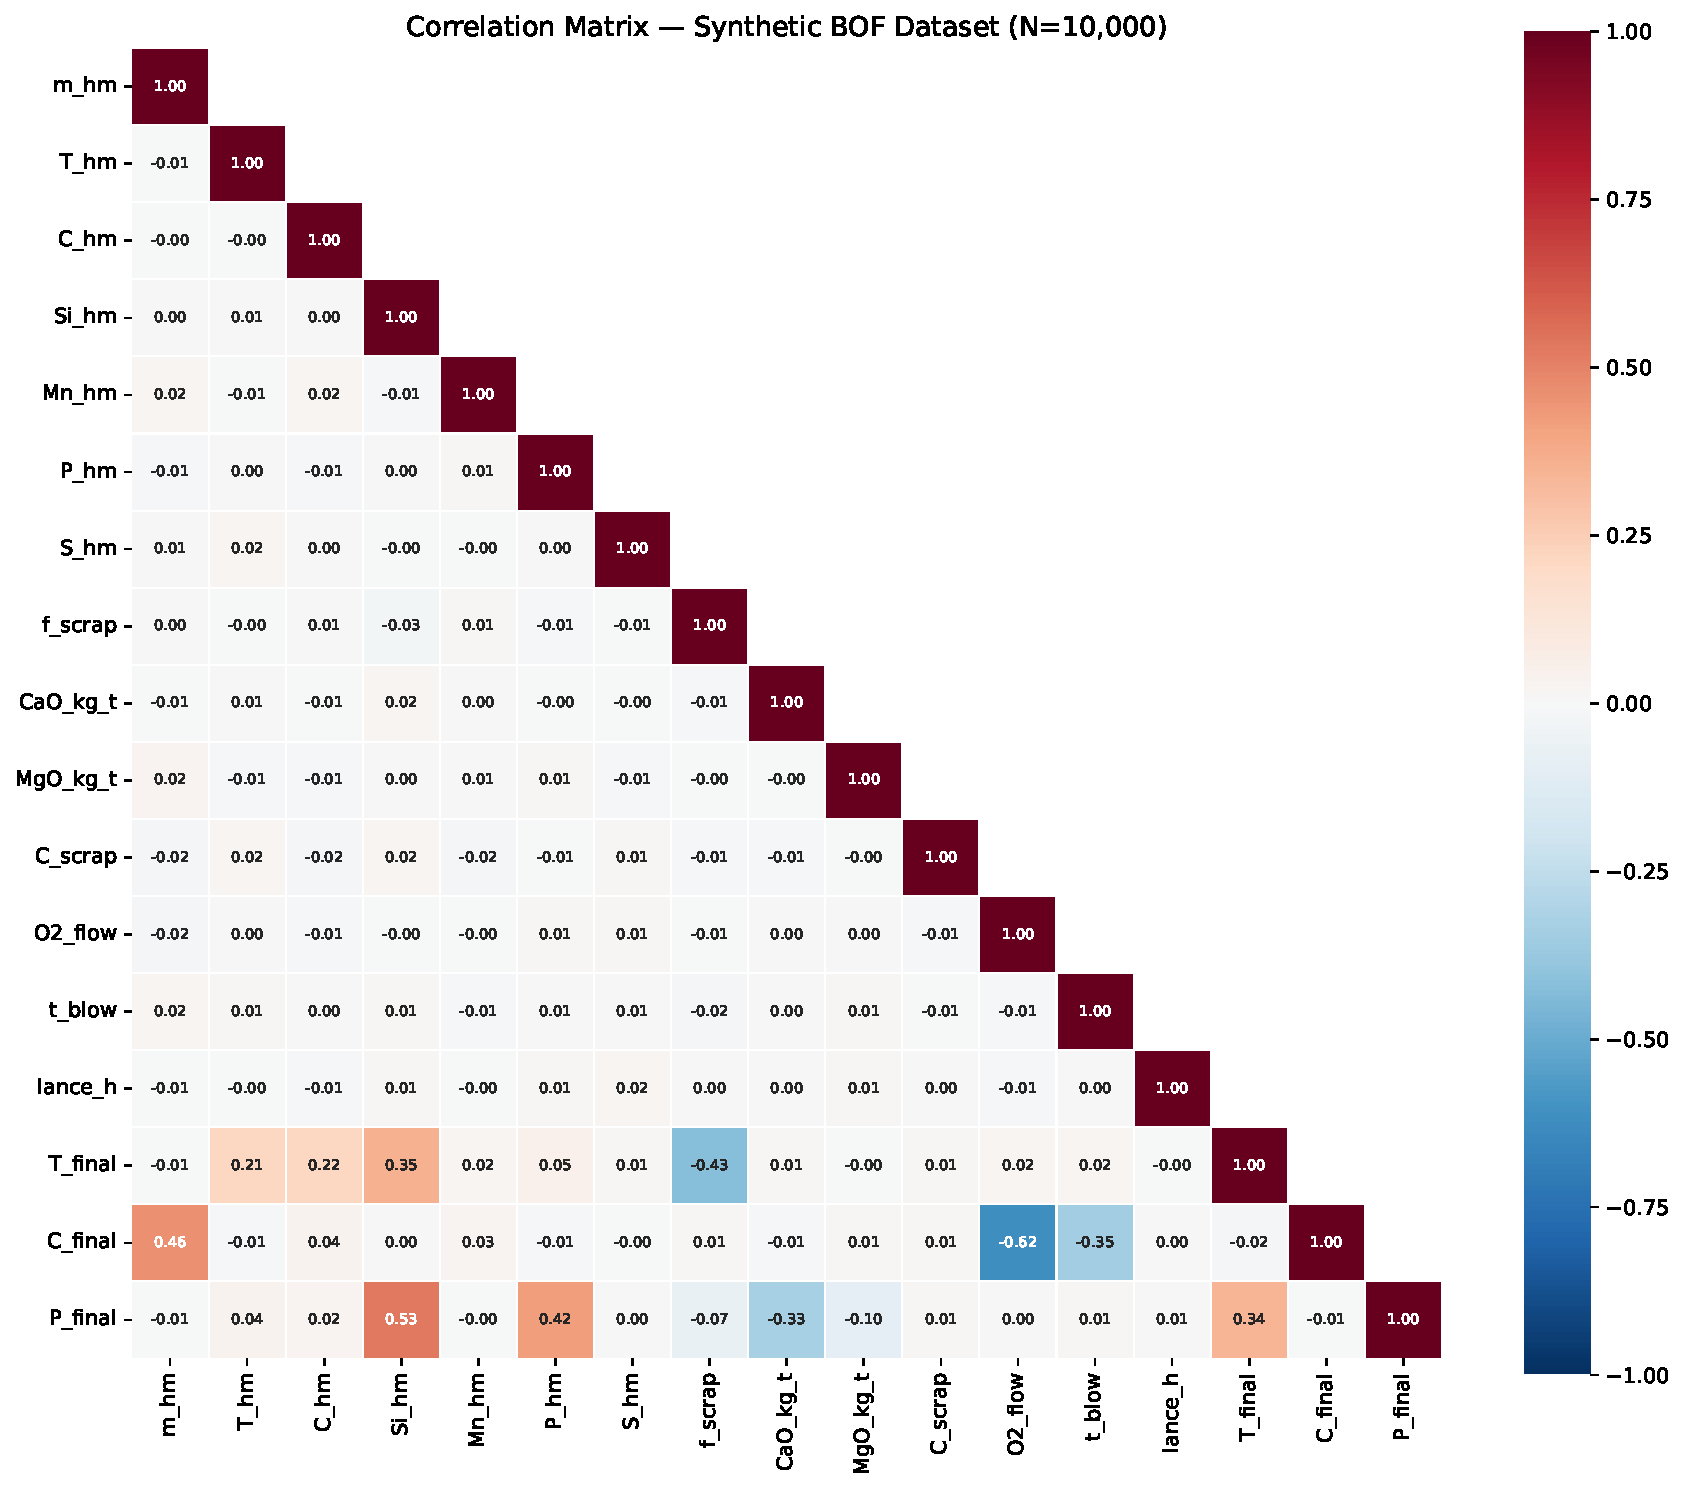
\includegraphics[width=0.82\textwidth]{Images/results/correlation_matrix.pdf}
\caption{Matriz de correlação (Pearson) do dataset sintético ($N = 10{.}000$): 14 variáveis de entrada e três alvos. As correlações mais fortes são fisicamente coerentes: $r(\texttt{O2\_flow}, [\text{C}]_\text{final}) = -0{,}62$ (mais O$_2$ remove mais C) e $r(\texttt{Si\_hm}, [\text{P}]_\text{final}) = +0{,}52$ (Si compete com P pela oxidação).}
\label{fig:corr_matrix}
\end{figure}

Os gráficos de dispersão predito vs.\ observado (Figuras~\ref{fig:predvsactual_C_cfinal} e \ref{fig:predvsactual_C_pfinal}) mostram a relação global entre predição e valor real; os gráficos de resíduo vs.\ predito (Figuras~\ref{fig:residuals_C_cfinal} e \ref{fig:residuals_C_pfinal}) são o diagnóstico apropriado para viés sistemático e heterocedasticidade, e complementam --- não substituem --- a leitura anterior. O CatBoost/Config~C para $[\text{C}]_\text{final}$ tem resíduo médio $\approx 0{,}0007\,\%$ (desprezível frente ao MAE de 0{,}0086\,\%) e correlação entre $|\text{resíduo}|$ e valor predito de apenas $0{,}017$, sem heterocedasticidade apreciável; o mesmo modelo para $[\text{P}]_\text{final}$ tem resíduo médio $\approx -0{,}0001\,\%$, mas correlação de $0{,}17$, indicando heterocedasticidade leve (erro absoluto maior para predições mais altas). Como no caso de $T_\text{final}$ (Seção~\ref{sec:resultados-A}), parte do $R^2$ de $[\text{C}]_\text{final}$ também é inflada pela censura nos limites da faixa-alvo: excluindo as amostras saturadas no conjunto de teste ($33{,}3\,\%$; a fração no dataset completo é $35{,}2\,\%$, Capítulo~\ref{chp:capitulo4}), o $R^2$ do CatBoost cai de $0{,}843$ para $0{,}766$, e o MAE sobe de $0{,}0086\,\%$ para $0{,}0101\,\%$ --- ainda um resultado sólido, mas a métrica sobre a amostra completa é, nesse caso, otimista tanto em $R^2$ quanto em MAE.

\begin{figure}[H]
\centering
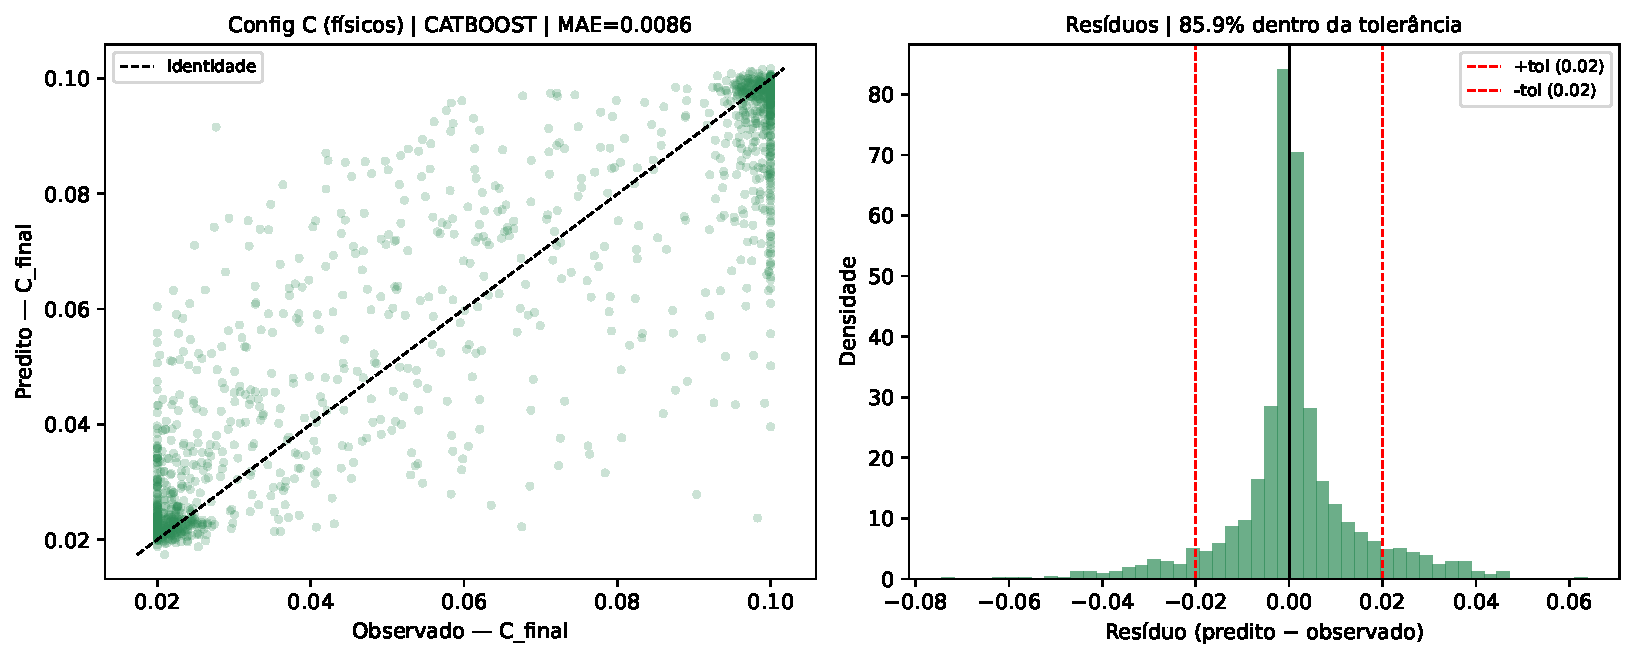
\includegraphics[width=0.75\textwidth]{Images/results/predvsactual_C_physics_catboost_C_final.pdf}
\caption{Predito vs.\ observado: CatBoost, Config~C, $[\text{C}]_\text{final}$. MAE = 0{,}0086\,\%, $R^2 = 0{,}843$.}
\label{fig:predvsactual_C_cfinal}
\end{figure}

\begin{figure}[H]
\centering
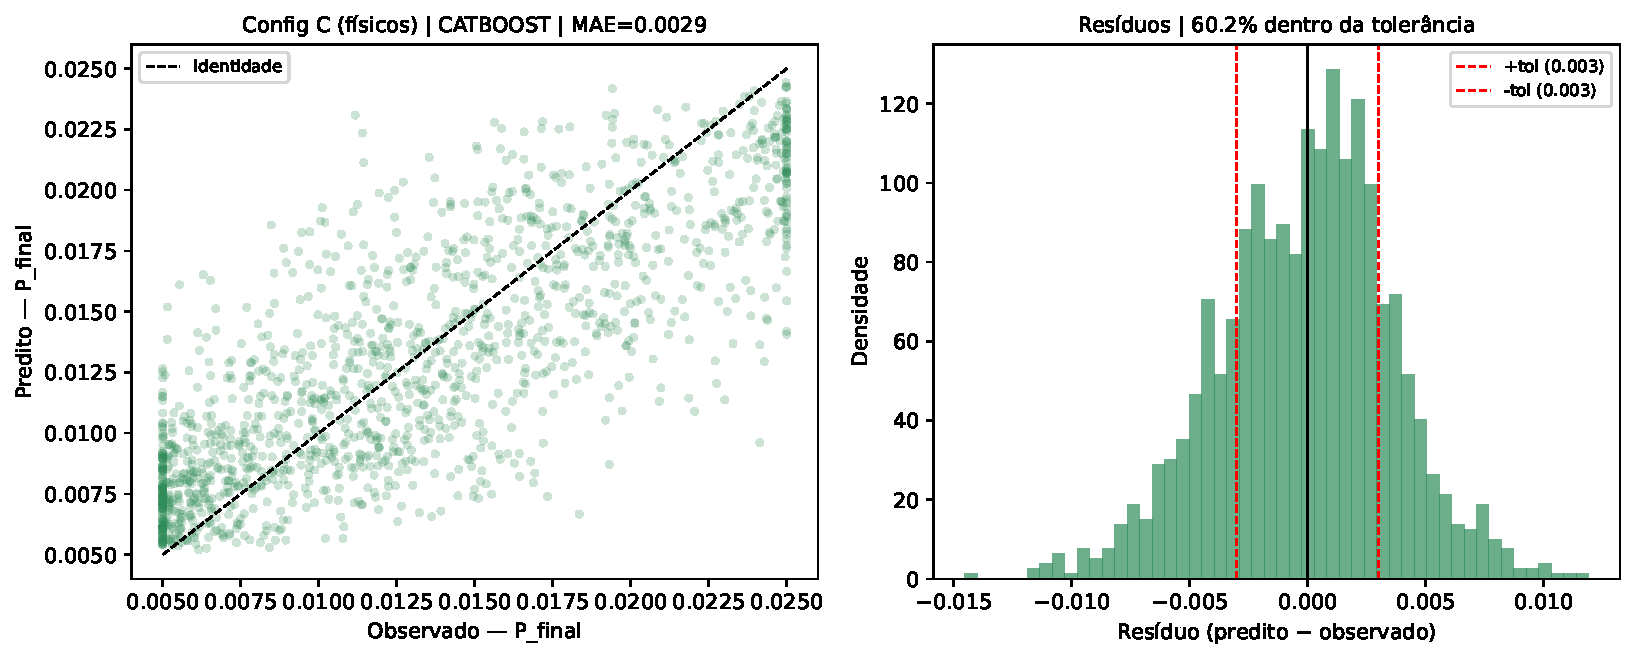
\includegraphics[width=0.75\textwidth]{Images/results/predvsactual_C_physics_catboost_P_final.pdf}
\caption{Predito vs.\ observado: CatBoost, Config~C, $[\text{P}]_\text{final}$. MAE = 0{,}0029\,\%, $R^2 = 0{,}664$.}
\label{fig:predvsactual_C_pfinal}
\end{figure}

\begin{figure}[H]
\centering
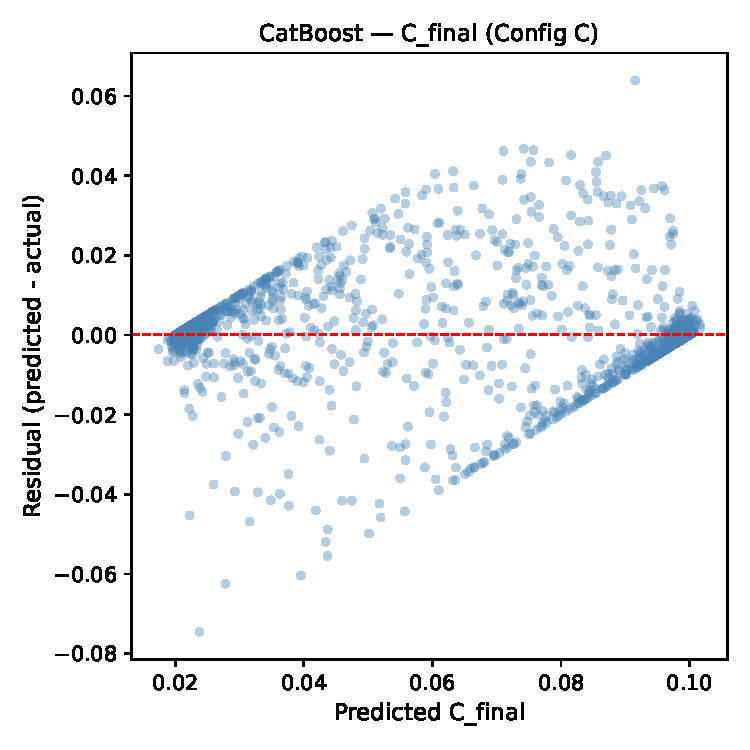
\includegraphics[width=0.75\textwidth]{Images/results/residuals_catboost_C_final.pdf}
\caption{Resíduo (predito $-$ observado) vs.\ predito: CatBoost, Config~C, $[\text{C}]_\text{final}$. Resíduo médio $\approx 0{,}0007\,\%$ (desprezível frente ao MAE de 0{,}0086\,\%) e correlação entre $|\text{resíduo}|$ e valor predito de apenas $0{,}017$: sem viés sistemático nem heterocedasticidade apreciável.}
\label{fig:residuals_C_cfinal}
\end{figure}

\begin{figure}[H]
\centering
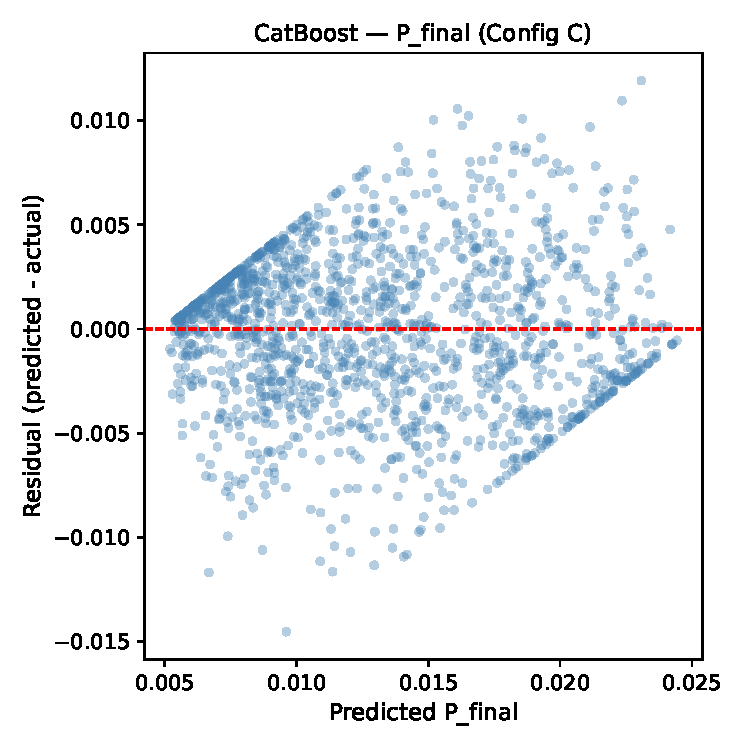
\includegraphics[width=0.75\textwidth]{Images/results/residuals_catboost_P_final.pdf}
\caption{Resíduo (predito $-$ observado) vs.\ predito: CatBoost, Config~C, $[\text{P}]_\text{final}$. Resíduo médio $\approx -0{,}0001\,\%$ (sem viés sistemático), mas correlação entre $|\text{resíduo}|$ e valor predito de $0{,}17$ --- heterocedasticidade leve, com erro absoluto ligeiramente maior para predições de $[\text{P}]_\text{final}$ mais altas.}
\label{fig:residuals_C_pfinal}
\end{figure}


\section{Análise de Interpretabilidade via SHAP}
\label{sec:shap-resultados}

A análise SHAP (SHapley Additive exPlanations) foi conduzida sobre três modelos representativos de famílias distintas da Config~C (RF, XGBoost, MLP --- ensemble de bagging, \textit{boosting} e rede neural, respectivamente) para cada alvo, utilizando TreeExplainer para os modelos de árvore e KernelExplainer com 200 amostras de fundo para o MLP\,\cite{lundberg2017unified,manojlovic2022eaf,xia2024dmpinn}. Esses três não são necessariamente os de menor MAE em cada alvo individualmente (Tabelas~\ref{tbl:resultados_configA}--\ref{tbl:resultados_configC}) --- notavelmente, o MLP é o pior modelo da Config~C para $T_\text{final}$ --- mas cobrem os principais paradigmas de modelo usados na comparação, o que é relevante para a leitura das hipóteses H1, H4 e H5 adiante, cuja média entre os três é por vezes dominada pelo modelo com maior magnitude de SHAP bruto, não pelo de melhor desempenho preditivo. A Tabela~\ref{tbl:shap_importance} apresenta as cinco features de maior importância média $|\text{SHAP}|$ por alvo, consolidadas como média aritmética dos três modelos.

\begin{table}[H]
\caption{Top-5 features por importância SHAP média $\overline{|\phi|}$ (média de RF, XGBoost, MLP da Config~C). Features físico-derivadas são marcadas com $\bullet$.}
\label{tbl:shap_importance}
\centering
\footnotesize
\setlength{\tabcolsep}{4pt}
\begin{tabular}{clrclrclr}
\hline
\multicolumn{3}{c}{$T_\text{final}$} & \multicolumn{3}{c}{$[\text{C}]_\text{final}$} & \multicolumn{3}{c}{$[\text{P}]_\text{final}$} \\
\cline{1-3}\cline{4-6}\cline{7-9}
\# & Feature & $\overline{|\phi|}$ & \# & Feature & $\overline{|\phi|}$ & \# & Feature & $\overline{|\phi|}$ \\
\hline
1 & \texttt{t\_blow}              & 87,07 & 1 & $\bullet$ \texttt{o2\_efficiency}  & 0,0195 & 1 & $\bullet$ \texttt{slag\_basicity} & 0,00282 \\
2 & $\bullet$ \texttt{o2\_efficiency}      & 73,69 & 2 & \texttt{O2\_flow}               & 0,0069 & 2 & \texttt{P\_hm}                   & 0,00228 \\
3 & $\bullet$ \texttt{decarb\_rate}        & 67,10 & 3 & $\bullet$ \texttt{fe\_oxidation\_loss}   & 0,0036 & 3 & $\bullet$ \texttt{theo\_o2\_demand}        & 0,00077 \\
4 & $\bullet$ \texttt{slag\_basicity}      & 51,91 & 4 & \texttt{t\_blow}                & 0,0027 & 4 & \texttt{Si\_hm}                  & 0,00062 \\
5 & \texttt{O2\_flow}            & 41,87 & 5 & \texttt{m\_hm}                  & 0,0023 & 5 & \texttt{m\_hm}                   & 0,00050 \\
\hline
\end{tabular}
\end{table}

A Tabela~\ref{tbl:shap_importance} mostra que features físico-derivadas ocupam posições relevantes para os três alvos: \texttt{o2\_efficiency} e \texttt{decarb\_rate} são as features \#2 e \#3 para $T_\text{final}$ (com a ressalva sobre agregação entre modelos discutida adiante); \texttt{o2\_efficiency} é a feature \#1 para $[\text{C}]_\text{final}$ no RF e no XGBoost, e \#2 no MLP (atrás de \texttt{O2\_flow}); e \texttt{slag\_basicity} é a feature \#1 para $[\text{P}]_\text{final}$, embora com margem modesta sobre a segunda posição --- indicando que a composição bruta do gusa continua sendo um preditor quase tão relevante quanto o atributo físico-derivado combinado. A Figura~\ref{fig:shap_beeswarm_cfinal} mostra o gráfico \textit{beeswarm} do XGBoost para $[\text{C}]_\text{final}$, confirmando que \texttt{o2\_efficiency} domina a predição com relação monotônica \emph{direta} --- maior \texttt{o2\_efficiency} corresponde a maior $[\text{C}]_\text{final}$ predito (SHAP médio assinado positivo nos três modelos), não o inverso: como \texttt{o2\_efficiency} = \texttt{theo\_o2\_demand} / (O$_2$\_soprado $\times$ tempo de sopro) e \texttt{theo\_o2\_demand} cresce com a carga inicial de impurezas do gusa, corridas com maior carga inicial produzem simultaneamente maior \texttt{o2\_efficiency} \emph{e} maior $[\text{C}]_\text{final}$ residual --- uma relação de causa comum, não de causalidade direta entre o atributo e o alvo.

\begin{figure}[H]
\centering
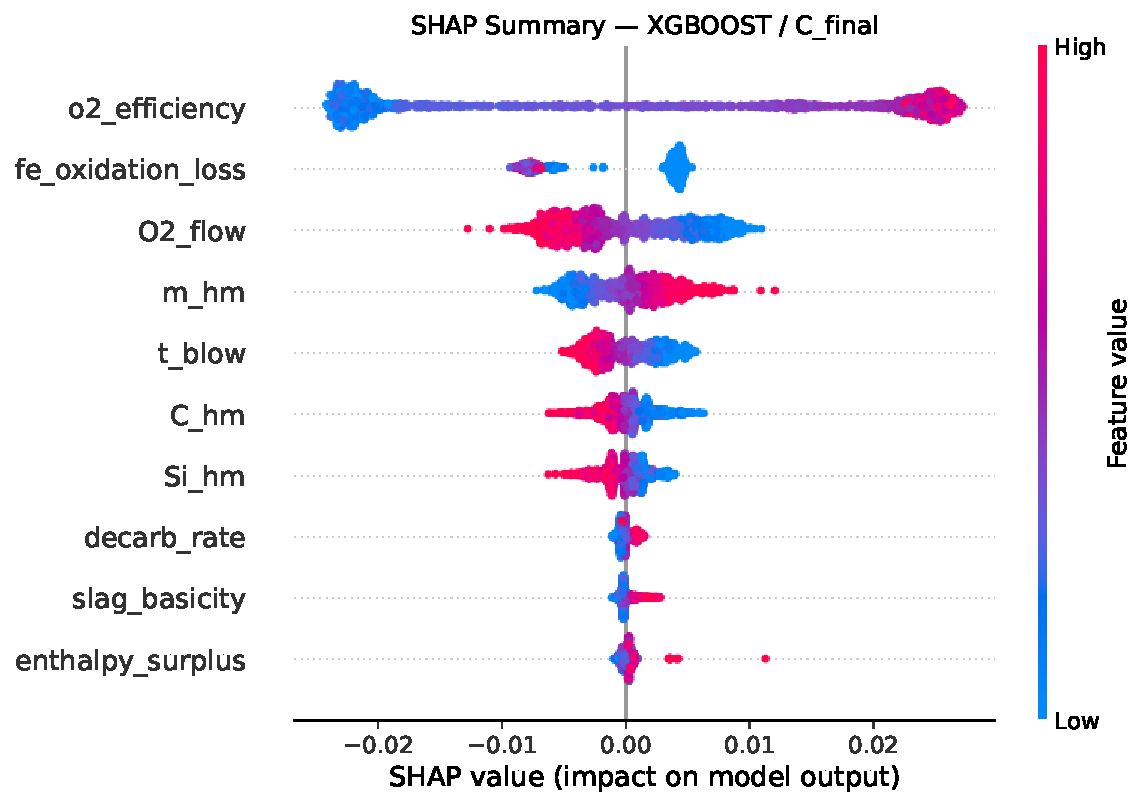
\includegraphics[width=0.85\textwidth]{Images/shap/summary_xgboost_C_final.pdf}
\caption{Gráfico \textit{beeswarm} SHAP do XGBoost (Config~C) para $[\text{C}]_\text{final}$. A feature \texttt{o2\_efficiency} (físico-derivada) domina, com importância $3{,}8\times$ superior à segunda posição neste modelo (\texttt{fe\_oxidation\_loss}); a relação é direta, não inversa (ver texto).}
\label{fig:shap_beeswarm_cfinal}
\end{figure}

\begin{figure}[H]
\centering
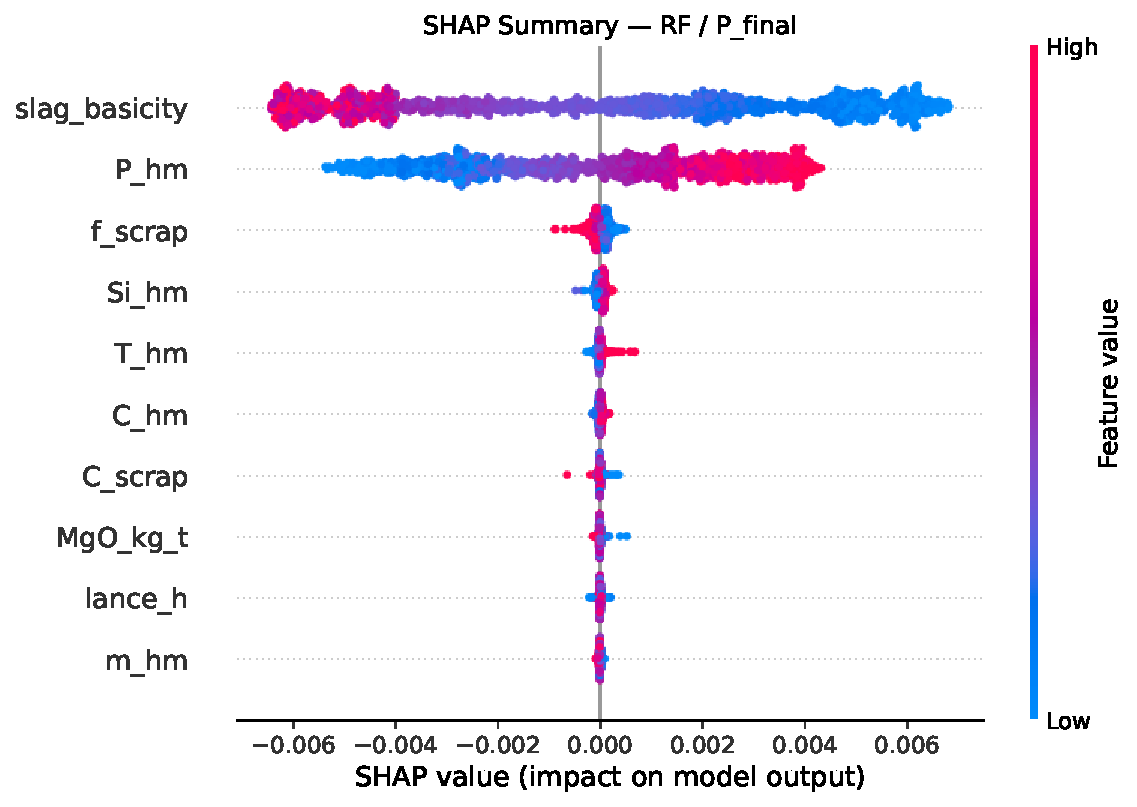
\includegraphics[width=0.85\textwidth]{Images/shap/summary_rf_P_final.pdf}
\caption{Gráfico \textit{beeswarm} SHAP do RF (Config~C) para $[\text{P}]_\text{final}$. \texttt{slag\_basicity} (físico-derivada) é a feature de maior importância, com margem modesta ($1{,}63\times$ neste modelo) sobre \texttt{P\_hm}, consistente com o mecanismo termodinâmico de desfosforação pela basicidade da escória~\cite{bae2020bof}.}
\label{fig:shap_beeswarm_pfinal}
\end{figure}

A Tabela~\ref{tbl:shap_hypotheses} reporta os resultados dos cinco testes de coerência física definidos no Capítulo~\ref{chp:capitulo4} (H1 e H2 aceitam \texttt{theo\_o2\_demand} \emph{ou} \texttt{o2\_efficiency} como satisfazendo a hipótese, conforme formulado no Capítulo~\ref{chp:capitulo1}; H4 e H5 são resolvidas pelo sinal médio do SHAP, não apenas por sua magnitude).

\begin{table}[H]
\caption{Resultados dos testes de hipótese de coerência física SHAP (H1--H5).}
\label{tbl:shap_hypotheses}
\centering
\footnotesize
\resizebox{\textwidth}{!}{%
\setlength{\tabcolsep}{4pt}
\begin{tabular}{cp{4.2cm}p{1.8cm}p{6.0cm}}
\hline
\textbf{H} & \textbf{Hipótese} & \textbf{Resultado} & \textbf{Evidência} \\
\hline
H1 & \texttt{theo\_o2\_demand} ou \texttt{o2\_efficiency} top-3 para $T_\text{final}$ & Confirmada na média, não por modelo individual & Top-3 médio: \texttt{t\_blow}, \texttt{o2\_efficiency}, \texttt{decarb\_rate}; mas apenas no MLP (2\textordmasculine) --- RF e XGBoost não incluem nenhum atributo de O$_2$ em seus próprios top-3 \\[3pt]
H2 & \texttt{theo\_o2\_demand} ou \texttt{o2\_efficiency} top-3 para $[\text{C}]_\text{final}$ & Confirmada por modelo individual & Top-3: \texttt{o2\_efficiency}, \texttt{O2\_flow}, \texttt{fe\_oxidation\_loss}; \texttt{o2\_efficiency} está no top-3 dos três modelos (\#1 em RF/XGBoost, \#2 no MLP) \\[3pt]
H3 & \texttt{slag\_basicity} top-3 para $[\text{P}]_\text{final}$ & Confirmada & \texttt{slag\_basicity} é \#1, mas com margem modesta sobre \texttt{P\_hm} \\[3pt]
H4 & \texttt{decarb\_rate} dir.\ negativa para $[\text{C}]_\text{final}$ & Confirmada na média, sinal divergente entre modelos & SHAP médio assinado $= -0{,}000114$; sinal positivo (oposto ao hipotetizado) no RF, negativo no XGBoost e no MLP (dominante na média) \\[3pt]
H5 & \texttt{enthalpy\_surplus} dir.\ positiva para $T_\text{final}$ & Refutada na média, sinal divergente entre modelos & SHAP médio assinado $= -1{,}45$; sinal positivo (hipotetizado) em RF e XGBoost, negativo e de magnitude dominante no MLP \\
\hline
\end{tabular}}
\end{table}

H2 é confirmada de forma robusta: \texttt{o2\_efficiency} = \texttt{theo\_o2\_demand} / (O$_2$\_soprado $\times$ tempo de sopro) está no top-3 para $[\text{C}]_\text{final}$ nos três modelos individualmente (\#1 no RF e no XGBoost, \#2 no MLP, atrás de \texttt{O2\_flow}), não apenas na média. H1 é confirmada apenas pelo critério pré-registrado de média entre modelos --- \texttt{o2\_efficiency} é a \#2 no top-3 médio para $T_\text{final}$ --- mas essa média é dominada pelo MLP: individualmente, RF e XGBoost não colocam nenhum atributo relacionado a O$_2$ em seus próprios top-3 para $T_\text{final}$ (Seção~\ref{sec:shap-resultados} discute por que agregar $|\phi|$ entre TreeExplainer e KernelExplainer sem normalização favorece o modelo de escala bruta maior). H1 deve, portanto, ser lida como confirmada pelo protocolo pré-registrado, mas frágil a essa escolha de agregação --- o mesmo problema metodológico identificado adiante para H4 e H5. Onde \texttt{o2\_efficiency} de fato domina (H2), a relação com o alvo é direta, não inversa: como discutido acima, ambos crescem juntos com a carga inicial de impurezas do gusa~\cite{chattopadhyay2022hybrid}.

H3 é confirmada: \texttt{slag\_basicity} é a feature de maior importância para $[\text{P}]_\text{final}$ --- o critério pré-registrado (top-3) é satisfeito com folga --- ainda que por margem modesta sobre \texttt{P\_hm} (o teor bruto de fósforo do gusa); isso é fisicamente sensato, já que o teor inicial de P é, por si só, um forte preditor de quanto restará após a remoção parcial\,\cite{bae2020bof,chattopadhyay2022hybrid}, e não contradiz a hipótese, que nunca postulou magnitude de dominância, apenas posição relativa.

H4 é confirmada apenas na média, com o mesmo padrão de fragilidade identificado para H1 e H5: o sinal assinado de \texttt{decarb\_rate} para $[\text{C}]_\text{final}$ é positivo no RF (o oposto do hipotetizado), negativo no XGBoost e fortemente negativo no MLP, que domina a média. A relação algébrica esperada é, de fato, ambígua a priori: $\texttt{decarb\_rate} = [\text{C}]_\text{hm} / t_\text{blow}$ e $[\text{C}]_\text{final} \propto [\text{C}]_\text{hm} \cdot \exp(-k \cdot r_{\text{O}_2})$ (Capítulo~\ref{chp:capitulo4}) --- um $[\text{C}]_\text{hm}$ maior eleva ambos simultaneamente (sinal positivo, como no RF), enquanto um $t_\text{blow}$ maior reduz \texttt{decarb\_rate} mas também prolonga a oxidação, reduzindo $[\text{C}]_\text{final}$ (sinal negativo, como no XGBoost e no MLP). Qual mecanismo domina depende de qual dos dois canais cada modelo pondera mais fortemente, não de uma direção termodinâmica única e inequívoca; a leitura mais honesta é que H4 captura uma associação estatística real, mas de direção dependente do modelo, e não uma relação causal de sinal único.

H5 é refutada na média dos três modelos, mas o resultado por modelo é menos unânime do que a média sugere: o SHAP médio assinado de \texttt{enthalpy\_surplus} para $T_\text{final}$ é positivo --- o sinal hipotetizado --- tanto no RF ($+0{,}032$) quanto no XGBoost ($+0{,}041$), e apenas o MLP mostra sinal negativo ($-4{,}43$); como o MLP usa KernelExplainer (valores aproximados sobre 200 amostras de fundo) em vez do TreeExplainer exato dos outros dois, e sua magnitude é de 1 a 2 ordens de grandeza maior nesta feature (comparado a $|\phi| = 0{,}22$ no RF e $0{,}71$ no XGBoost), a média simples de três modelos é dominada por um único valor de magnitude e método de cálculo distintos. Em qualquer leitura, \texttt{enthalpy\_surplus} tem importância baixa para $T_\text{final}$ (13\textordmasculine\ de 22 atributos por $|\phi|$ médio, Seção~\ref{sec:shap-resultados}), de modo que H5 --- confirmada ou refutada --- não afeta a conclusão central de que $T_\text{final}$ permanece dominado por variância irredutível não capturada por nenhum atributo disponível. Uma explicação plausível para o sinal negativo específico do MLP é a de que \texttt{enthalpy\_surplus} é calculado com constantes fixas e frações de oxidação teóricas completas (Nível~2, §\,\ref{subsec:ameacas-validade}), enquanto $T_\text{final}$ é gerado com eficiência térmica e frações de remoção específicas à corrida ($\eta_\text{eff}$, Nível~1); esta é uma leitura pós-hoc, não uma hipótese testada de forma independente, e fica registrada como direção de investigação futura em vez de explicação definitiva.

Em síntese, a análise SHAP é consistente com os modelos da Config~C utilizando os atributos físico-derivados como vetores relevantes de predição, com quatro das cinco hipóteses de coerência física não falsificadas; a exceção (H5) mostra sinal dependente do modelo (positivo em RF e XGBoost, negativo e dominante no MLP) sobre um atributo de importância já baixa para $T_\text{final}$, o que por si só é um resultado informativo sobre os limites de agregar SHAP entre modelos com métodos de explicação distintos.


\section{Comparação com a Literatura}
\label{sec:comparacao-literatura}

Os ganhos observados na Config~C podem ser contextualizados frente aos resultados reportados na literatura de predição de ponto final BOF, reconhecendo que diferenças em dados (sintéticos vs.\ industriais), escalas de planta e variáveis de entrada tornam a comparação qualitativa e não direta.

\citeonline{bae2020bof} reportam que a adição de 17 atributos termodinâmicos a uma rede neural para predição de $T_\text{final}$ em dados reais de planta eleva a taxa de acerto dentro de $\pm 10\,^\circ\text{C}$ em 2--4 pontos percentuais (os autores não reportam um MAE absoluto de referência). Nesta dissertação, o ganho em $w_\text{tol}$ da Config~C sobre a Config~A para $T_\text{final}$ é nulo ou levemente negativo (o melhor modelo pareado, SVR, cai de $35{,}9\,\%$ para $34{,}5\,\%$). A diferença crucial é que \citeonline{bae2020bof} incluem medições de sublança intermediárias como atributos, enquanto esta dissertação restringe-se a variáveis pré-sopro --- um cenário informacionalmente mais restritivo. Como referência de MAE absoluto no mesmo regime pré-sopro (sem off-gas), \citeonline{zhou2024bof} reportam $7{,}96\,^\circ\text{C}$ (LightGBM, 45 variáveis tabulares) --- inferior aos $21{,}86$--$27{,}37\,^\circ\text{C}$ desta dissertação, refletindo o benefício de dados reais de planta e um conjunto de atributos tabulares mais amplo.

Para $[\text{C}]_\text{final}$, \citeonline{zhou2024bof} reportam MAE de $6{,}92\times10^{-3}\,\%$ com CatBoost sobre dados reais de planta, também no regime tabular sem off-gas (o modelo combinado com off-gas dos mesmos autores reduz esse valor a $6{,}41\times10^{-3}\,\%$ em teste, mas usa informação temporal indisponível nesta dissertação). O melhor resultado da Config~C (CatBoost, MAE~$= 0{,}0086\,\%$) é cerca de $24\,\%$ maior --- ou seja, pior --- que o valor tabular de \citeonline{zhou2024bof}, mesmo com o alvo desta dissertação já se beneficiando de uma proporção maior de amostras saturadas na faixa (\S\,\ref{sec:diagnostico-visual}). A diferença é plausivelmente explicada tanto pelo conjunto de atributos tabulares mais amplo de \citeonline{zhou2024bof} ($45$ variáveis, contra $22$ nesta dissertação) quanto pelo fato de que os alvos provêm de distribuições distintas --- uma gerada por um modelo físico simplificado sem os modos de falha, ruído de processo e não-linearidades de uma planta real, a outra medida diretamente em operação --- de modo que a proximidade ou distância numérica entre os MAE não deve ser lida como evidência de equivalência ou inferioridade metodológica entre as abordagens~\cite{shao2024hybrid}.

Para $[\text{P}]_\text{final}$, \citeonline{chattopadhyay2022hybrid} reportam que modelos híbridos serial (físico + ML) atingem MAE $\approx 0{,}004\,\%$ em dados reais, e a Config~C obtém 0{,}0029\,\% com CatBoost --- valor numericamente menor, mas obtido sobre dados sintéticos sem a complexidade total de uma planta real, o que impede tratar a comparação como evidência de superioridade\,\cite{buggineni2024synthetic}. A Tabela~\ref{tbl:comparacao_literatura} consolida essa comparação.

\begin{table}[H]
\caption{Contextualização do MAE desta dissertação frente à literatura. $\dagger$: dados sintéticos; demais: dados industriais reais. Os valores \textbf{não são diretamente comparáveis}: diferenças em escala de planta, variáveis disponíveis e, sobretudo, na natureza dos dados (sintéticos vs.\ reais) impedem inferir superioridade ou equivalência a partir da proximidade numérica.}
\label{tbl:comparacao_literatura}
\centering
\footnotesize
\setlength{\tabcolsep}{4pt}
\begin{tabular}{llrrp{3.8cm}}
\hline
\textbf{Alvo} & \textbf{Estudo} & \textbf{MAE} & \textbf{Modelo} & \textbf{Observação} \\
\hline
$T_\text{final}$ (°C) & \citeonline{zhou2024bof} & 7,96 & LightGBM & 45 var.\ tabulares, dados reais \\
 & Esta dissert.$^\dagger$ & 21,86 & SVR (A) & Apenas variáveis pré-sopro \\
\hline
$[\text{C}]$ (\%) & \citeonline{zhou2024bof} & 0,00692 & CatBoost & 45 var.\ tabulares, dados reais \\
 & Esta dissert.$^\dagger$ & 0,0086 & CatBoost (C) & 8 features físicas estáticas \\
\hline
$[\text{P}]$ (\%) & \citeonline{chattopadhyay2022hybrid} & $\approx$0,004 & Híbrido & Serial (físico+ML), dados reais \\
 & Esta dissert.$^\dagger$ & 0,0029 & CatBoost (C) & 8 features físicas estáticas \\
\hline
\end{tabular}
\end{table}

A engenharia de atributos físico-derivados produz, em suma, ganhos estatisticamente significativos e de relevância prática para $[\text{C}]_\text{final}$ (10 dos 11 modelos) e para $[\text{P}]_\text{final}$ (8 dos 11 modelos, com seis passando a atender ao limiar industrial contra apenas um na linha de base), mas não resolve o gargalo estrutural de $T_\text{final}$, cujo erro é dominado por variância irredutível do processo e pela ausência de informação temporal. O teste de extrapolação, além disso, mostra que esses ganhos para $[\text{C}]_\text{final}$ e $[\text{P}]_\text{final}$ se mantêm --- e no caso do fósforo, permanecem dentro do limiar industrial --- sob a extensão moderada de faixa de amostragem testada. A hipótese central da dissertação é, portanto, parcialmente confirmada: os atributos físico-derivados melhoram a predição frente à linha de base nos dois alvos com relação física mais direta com as features propostas, e esse benefício não desaparece sob a extrapolação testada, mas depende do alvo, da família de modelo utilizada e da informação disponível no momento da predição.

Toda essa avaliação, cabe reiterar, ocorre sobre dados sintéticos gerados por um modelo físico simplificado, não sobre uma planta real (Capítulo~\ref{chp:con}, Seção~\ref{sec:limitacoes}); os ganhos relativos entre configurações são internos ao universo do gerador e quantificam o valor da engenharia de atributos dentro dele, não necessariamente a magnitude que se observaria em dados industriais reais. A validação com dados de planta permanece, portanto, condição necessária antes de qualquer inferência sobre aplicabilidade operacional.
